\chapter{Experiments and results}\label{chap:exp_res}
This chapter evaluates the proposed method on toy data which consists of $128$ by $128$ pixel images including $6$ to $10$ disks of radii between $6$ and $8$ that are non overlapping but might be touching. The images are single channel and the disks are separating themselves from the background by phase shiftet, interfering frequencies. An example is depicted in figure \ref{fig:exmpl}.

\begin{figure}[ht!]
	\centering
	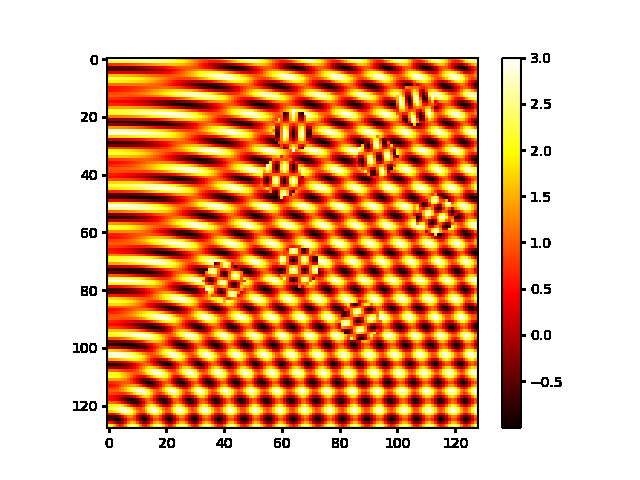
\includegraphics[width=.5\textwidth]{figures/plots/raw.png}
	\caption{Example raw data image}
	\label{fig:exmpl}
\end{figure}

The incentive is to do instance segmentation for the disks. That is, labeling each of the discs in a unique object ID. There are some foreground background segmentations created along with the raw data. These segmentations are used to train the embedding network as described in section \ref{seg:pip_embed}. Training the embedding network on foreground background images with contrastive loss generates two clusters only in the embedding space, one for foreground and one for background. For the node features $\vec{x}^0_i$ it is only important to be distinctive between those two classes because that is all the information needed for a merge/unmerge decision.\\
The pixel embeddings are visualized by their values in the first three principal components (see section \ref{sec:pca}) of the whole set of pixel embeddings. The three values per pixel are converted to a rgb-image. This is usually a sufficiently expressive visualization for pixel embeddings because for most trained pixel embeddings the vast majority of the information is contained within the first three principal components. In figure \ref{fig:pixembeddings} this visualization method is used for the pixel embeddings of the example image.\\

\begin{figure}[ht!]
	\centering
	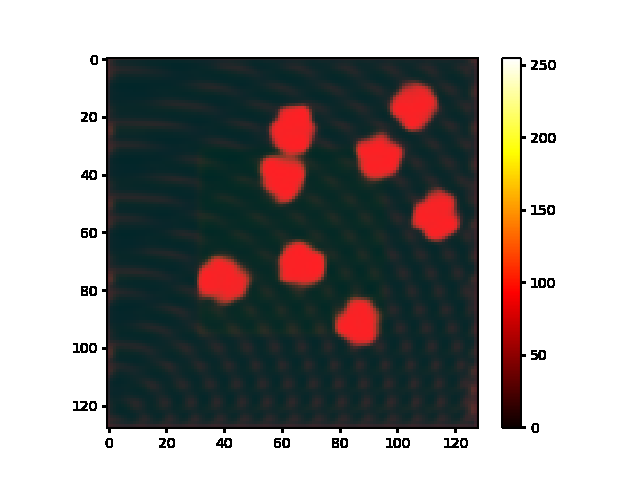
\includegraphics[width=.5\textwidth]{figures/plots/pix_embeddings.png}
	\caption{Projections of pixel embeddings to their first three principal components}
	\label{fig:pixembeddings}
\end{figure}

The affinities that are needed for the Mutex Watershed algorithm are calculated based on the fist gradient of the raw data for short range attractive edges. For long lange repulsive edges the concept of the gradient computation by forward differences is used for pixelwise differences between the incidental pixels (nodes) of the long range edges.\\
The algorithm mainly tested on this data operates in a continuous action space where the actor predicts mean and variance for a normal distribution sitting on every edge of the superpixel graph. The rewards are calculated in a supervised fashion based on the ground truth segmentation and in an unsupervised fashion based on the number of objects and the shape prior.\\
\subsection{Supervised training}
For the supervised method a reward per subgraph is obtained by the dice score over the set of edges in the subgraph and the ground truth edges. Ground truth edges are obtained from the ground truth foreground background segmentation by assigning $1$ to the edge if the larger parts of the incidental superpixels are of different classes in the ground truth segmentation and $0$ otherwise. The larger parts are taken here because it is not guaranteed that the superpixels do not cross edges in the ground truth segmentation.\\
The setup includes a replay buffer storing $100$ experience tuples of $(s_t, a_t, r_{t}, s_{t+1})$. Initially experience is sampeld until the buffer is full. Then after each collected experience tuple there are $10$ optimization steps performed on sampled experience tuples. The number of edges in each subgraph is set to $l=10$. Optimization is done by stochastic gradient descent on mini batches of size $10$ using the Adam optimizer, introduced in \cite{kingma2014adam}.\\
For the setting where the embedding network is pre-trained on raw image ground truth pairs, the embedding network's parameters remain fixed afterwards. The optimization of the embedding network by the actors optimizer and loss function has been tested, but could not be brought near to a adequate result. This can be related to high variance in the actors loss function.\\
An example of the result using the per subgraph dice score as a reward is shown in figure \ref{fig:resa_dice}.\\

\begin{figure}[ht!]
	\centering
	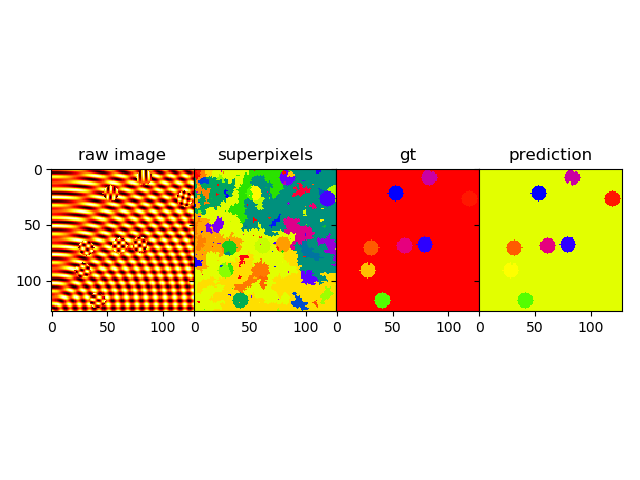
\includegraphics[width=.7\textwidth]{figures/plots/results_dice_reward.png}
	\caption{Result using the dice reward after $80000$ optimization steps on mini batches of size $10$. The gt image was obtained by the Multicut algorithm based on the ground truth edges}
	\label{fig:resa_dice}
\end{figure}

The values in their first three principal components of the edge features $\vec{e}_{ij}^M$, extracted from one of the critic's networks are displayed in figure \ref{fig:res_edge_embed}. After training they clearly carry the ground truth information.\\

\begin{figure}[ht!]
	\centering
	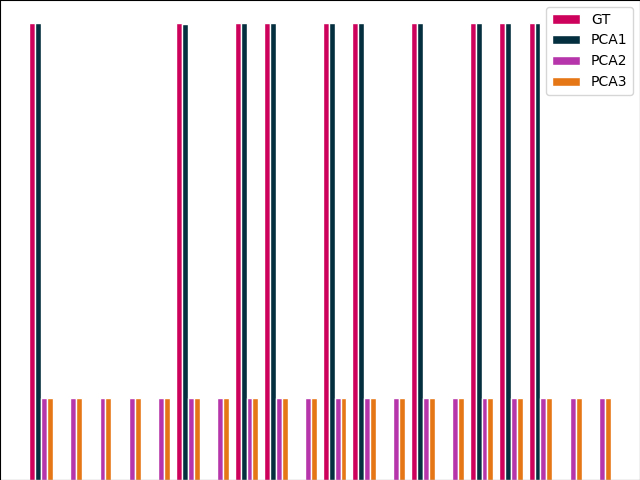
\includegraphics[width=.5\textwidth]{figures/plots/edge_embeddings.png}
	\caption{Visualization of the values of the edge features in their first three principal components (PCA1-3) and the ground truth edge values (GT) after training with the dice rewards for $80000$ optimization steps on mini batches of size $10$.}
	\label{fig:res_edge_embed}
\end{figure}

The predicted means of the actor network are visualized by histograms in figure \ref{fig:pred_means}. They are separated with a low uncertainty into means larger than $1$ and smaller than $0$. It also shows the class imbalance of $0$- and $1$-edges. The separation shows, that there is almost no uncertainty in the predictions anymore, leaving the Multicut algorithm with a comparatively simple task.

\begin{figure}[ht!]
	\centering
	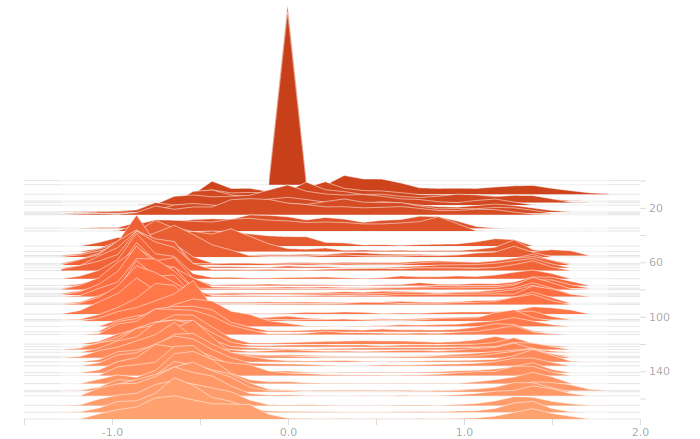
\includegraphics[width=.7\textwidth]{figures/plots/logit_means_hist.png}
	\caption{History of predicted means for the policy (supervised reward setting)}
	\label{fig:pred_means}
\end{figure}

\subsection{Unsupervised training}

Since there is still some ground truth involved in the warmup training for the feature extractor, this setup cannot be considered fully unsupervised. However there is no more ground truth involved in obtaining the rewards which is a large decline in supervision. The rewards are calculated locally on superpixel basis as well as globally in the following fashion.\\
For the segmentation obtained from the Multicut algorithm, objects larger than $32^2$ pixels are considered background and all remaining objects are considered foreground. If there are too little foreground objects (number of objects is part of prior knowledge) then all superpixels covered by background objects receive a negative reward. If there are too many objects, all the superpixel covered by foreground objects receive a negative reward.\\
Added to those global rewards is a score for the shape of the foreground objects. This is obtained by using the Circle Heugh transform (CHT) (see section \ref{ssec:heugh_tf}). The CHT for all possible radii (part of prior knowledge) is applied on the edge image of the corresponding segmentation. All superpixels that are covered by discs that are drawn at the cells (pixels) of the Heugh transform above a threshold of $0.8$ receive a positive reward dependending on the value on the CHT score at the discs center.\\
In a final step the rewards are collected over each subgraph and averaged to a single value. This method generates quite noisy rewards but the proposed pipeline is able to compensate for that.\\
An example edge image and the respective CHT of a segmentation during training is shown in figure \ref{fig:seg_heugh}. The reward landscape for a foreground superpixel is shown in figure \ref{fig:ret_land}. A small value is added to the global reward if the number of foreground objects is within the accepted range. Figure \ref{fig:resa_unsup} shows an example of the results where the policy was trained using the unsupervised rewards.
\begin{figure}[ht!]
	\centering
	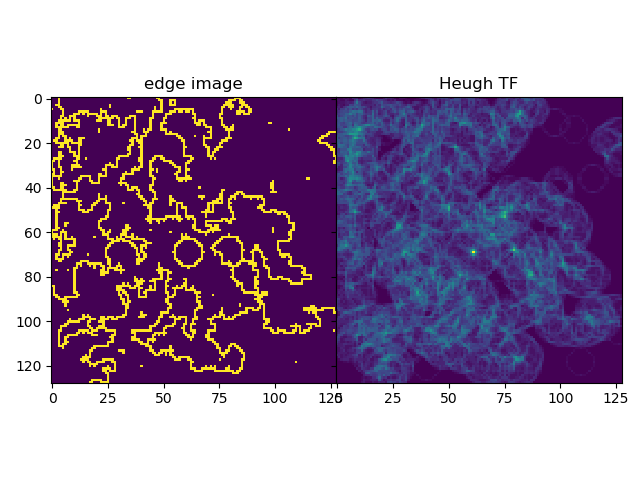
\includegraphics[width=.8\textwidth]{figures/plots/bad_seg_edge_heugh.png}
	\caption{Example edge image and respective CHT}
	\label{fig:seg_heugh}
\end{figure}
\begin{figure}[ht!]
	\centering
	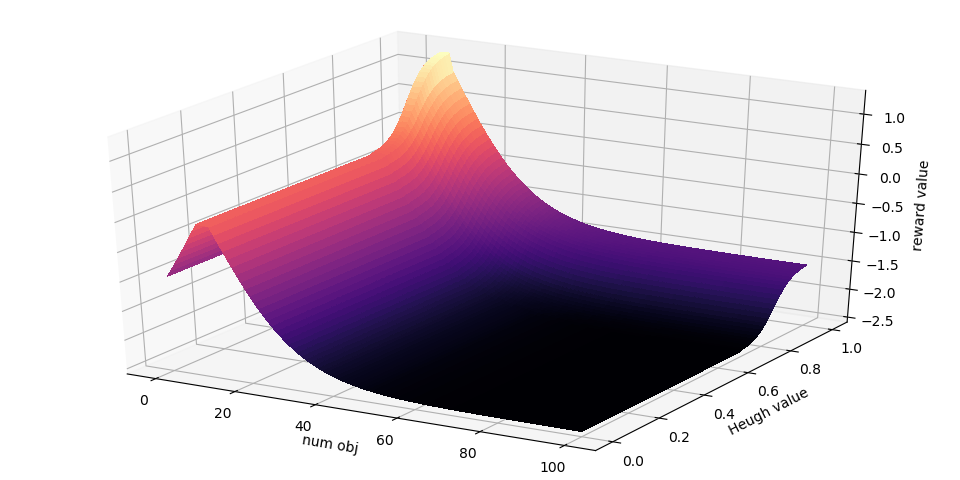
\includegraphics[width=.8\textwidth]{figures/plots/return_landscape.png}
	\caption{Reward landscape for a foreground superpixel that is covered by a circle with a corresponding CHT value.}
	\label{fig:ret_land}
\end{figure}
\begin{figure}[ht!]
	\centering
	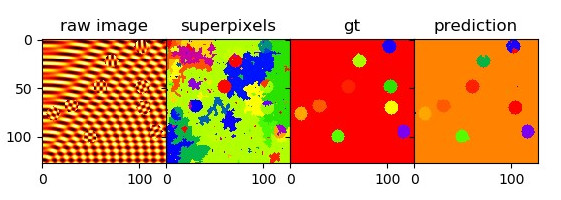
\includegraphics[width=.8\textwidth]{figures/plots/res_unsup.jpeg}
	\caption{Result using the unsupervised reward after $80000$ optimization steps on mini batches of size $10$. The gt image was obtained by the Multicut algorithm based on the ground truth edges}
	\label{fig:resa_unsup}
\end{figure}
As the histogram of the predicted means for the policy in figure \ref{fig:resa_unsup_hist} shows, the predictions are not so clearly separated into means that are larger than $1$ or smaller than $0$ as is the case in the supervised setting. This can be attributed to the noisy rewards and leaves the Multicut algorithm with a harder problem than in the supervised setting.\\
\begin{figure}[ht!]
	\centering
	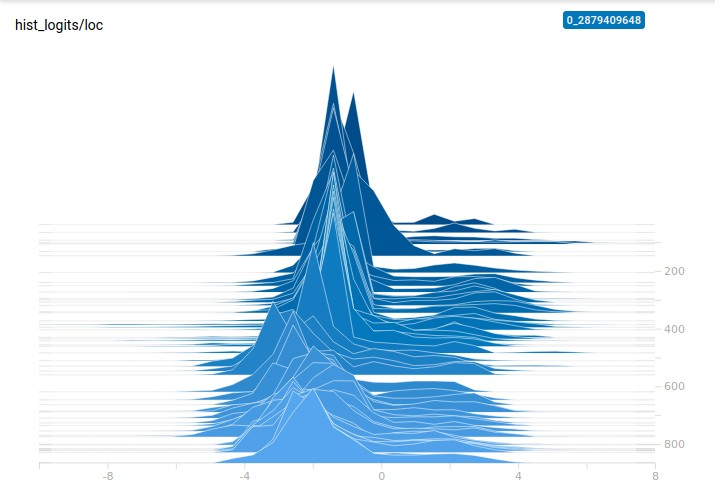
\includegraphics[width=.6\textwidth]{figures/plots/hist_unsup.jpeg}
	\caption{History of predicted means for the policy (unsupervised reward setting)}
	\label{fig:resa_unsup_hist}
\end{figure}

\subsubsection{Data conformity}
Supervised learning naturally provides a strict relation to the input data because the ground truth sample depends directly on the raw data.\\
Unsupervised learning typically needs a data term that encourages the solution to be close to the true labels of the input data. The data term in this pipeline is induced by the affinities and therefore the superpixel segmentation as well as by the pixel embeddings when the parameters of the embedding network remain fixed after pre-training. The policy network learns ideally to distinguish between disc and non-disc superpixels. In an unfortunate case however it also could learn to build disks out of background superpixels. This would be the case if the shape of each superpixel is encoded in the pixel embeddings and the policy network learns to build discs based only on these shapes. Preventing the prediction being dependent on the superpixel shapes can be done by removing the edge image of the superpixel segmentation from the state $s_t$ and therefore from the input to the embedding network.\\
Affinities can also be obtained from pixel embeddings that where optimized by the contrastive loss. Doing that produces less superpixels because these semantic affinities are based on object and non-object relations rather than on differences in pixel intensities of the raw data. This only makes sense if there is some ground truth which the emebdding network can be optimized with, using contrastive loss. However after that, the parameters of the embedding network should not be trained on unsupervised signals because the affinities are dependent on the pixel embeddings which are the only remaining data dependency. Changing the embeddings based on an unsupervised signal that inherits no data term might cause the affinities do not represent the data anymore.\\
There have also be some thoughts of obtaining superpixels by clustering pixels directly in the embedding space using the Mean Shift algorithm \cite{400568} which is differentiable. This adds some degrees of freedom to the differentiability w.r.t the superpixel generation but also comes with the downside of loosing the data term within the affinities.\\



